\chapter{Problemdefinition und Zielkriterien}\label{ch:problemdefinition-und-zielkriterien}

\textcolor{orange}{// TODO Hier Hier fehlt noch etwas der Bezug zu der vorher gut vorgestellten Domäne. Wahrscheinlich schafft das Kapitel "Verwandte Arbeiten" da noch einen besseren Übergang}

Dieses Kapitel präzisiert die Aufgabe der Arbeit, die Qualitätsziele der Klassifikation und steckt den fachlichen Geltungsbereich ab. Außerdem wird das Experimentdesign beschrieben, um die Forschungsfragen systematisch zu beantworten. Damit schafft es die Grundlage für die in Kapitel~\ref{ch:klassifizierungsalgorithmus-(design-und-implementierung)} beschriebene Klassifizierungspipeline sowie für die späteren Experimente und deren Auswertung.

Abbildung \ref{fig:running_example} zeigt einen Beispielprozess, der in den folgenden Abschnitten als laufendes Beispiel dient. Er modelliert den Versand eines Statusberichts eines Onlineshops an Kunden. Dabei werden personenbezogene Daten in den Aktivitäten \enquote{Tracking-id generieren} und \enquote{Status Update senden} verarbeitet, die die stabilen \texttt{ids} \texttt{Activity\_generate} und \texttt{Activity\_send} besitzen. Die Aktivität \enquote{Benachrichtigungsvorlage laden}, mit der \texttt{id} \texttt{Activity\_template}, dient als Negativbeispiel.

\begin{figure}[h]
    \centering
    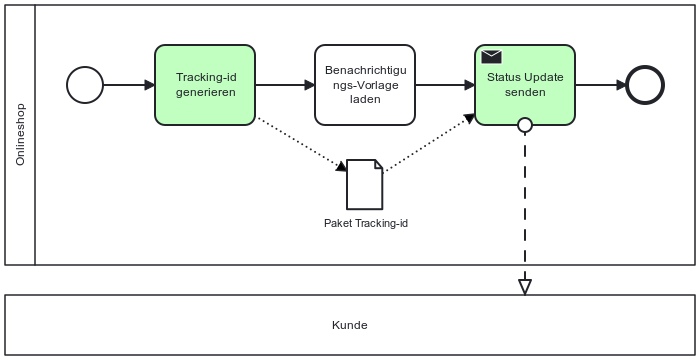
\includegraphics[width=0.7\textwidth]{images/running_example}
    \caption{Beispielprozess zur Veranschaulichung der Aufgabenstellung}
    \label{fig:running_example}
\end{figure}

\section{Aufgabenstellung}\label{sec:aufgabenstellung}

Ziel der Arbeit ist eine \emph{binäre Klassifikation} auf Ebene einzelner \ac{BPMN}-Aktivitäten: Für jede Aktivität eines Eingabemodells im \ac{BPMN}-XML-Format (Version 2.0.2) \cite{omgbpmn} soll entschieden werden, ob sie \emph{kritisch} im Sinne des Datenschutzrechts ist oder nicht.

\begin{itemize}
    \item \textbf{Eingabe} ist ein valides \ac{BPMN}-XML mit stabilen \texttt{id}-Attributen je Aktivität \cite{omgbpmn}.
    \item \textbf{Ausgabe} ist eine Menge von Aktivitäts-\texttt{ids}, die als \emph{kritisch} klassifiziert worden sind. Optional kann zusätzlich eine natürlichsprachige Begründung für einzelne Entscheidungen ausgegeben werden. Im Fall der Klassifizierungspipeline dieser Arbeit werden die Begründungen vom \ac{LLM} generiert. Die Erklärungen dienen ausschlißelich der Nachvollziehbarkeit der gewählten Klassifizierungen, werden allerdings nicht in der Evaluation berücksichtigt.
\end{itemize}

\subsection*{Begriffsbestimmung \enquote{kritisch}}

Eine Aktivität gilt in dieser Arbeit als \emph{kritisch}, wenn sie \emph{personenbezogene Daten} verarbeitet.Nach Art.~4~Abs.~1 \ac{DSGVO} sind personenbezogene Daten alle Informationen, die sich auf eine identifizierte oder identifizierbare natürliche Person beziehen, und \emph{Verarbeitung} umfasst gemäß Art-~4~Abs.~2 jede mit personenbezogenen Daten vorgenommene Operation (u.\,a. Erheben, Speichern, Abrufen, Verwenden, Übermitteln, Löschen) \cite{GDPR2016}. Dies schließt auch die \emph{Nutzung bereits vorhandener Daten} (z.\,B. Lesen/Abgleichen) ein.
Die Aufgabenstellung reiht sich damit in verwandte Arbeiten ein, die kritische/unkritische Tätigkeiten in Prozessartefakten kennzeichnen (z.\,B. für textuelle Prozessbeschreibungen) \cite{nake2023towards}.
\section{Qualitätsziele}\label{sec:qualitatsziele}

Die Aufgabe der datenschutzrechtlichen Klassifikation von Prozessen ist risikosensitiv. Übersehene kritische Aktivitäten, auch \acp{FN} genannt, bergen erhebliche Compliance-Risiken und können zu hohen Strafen nach der \ac{DSGVO} führen. Beispielsweise erhielt Meta Platforms Ireland Limited (Meta IE) 2023 aufgrund von rechtswidriger Übermittlung von \ac{EU} Nutzerdaten in die USA eine Geldbuße von 1,2 Milliarden Euro \cite{edpb-meta-fine}. Auch Amazon wurde 2025 nach einem langjährigen Rechtsstreit wegen Datenschutzverstößen mit 746 Millionen Euro bestraft \cite{datenschutzticker-amazon-fine, reuters-amazon-fine}. Um derartige Strafen zu vermeiden, müssen kritische Aktivitäten zuverlässig identifiziert werden. Daher ist das \textbf{Hauptziel} der Klassifikation:

\begin{hauptzielbox}
    \textbf{Maximaler Recall} bei \emph{minimalen \acp{FN}} und zugleich \emph{akzeptabler Precision}, damit der manuelle Prüfaufwand durch \acp{FP} begrenzt bleibt.
\end{hauptzielbox}

\subsection*{Konfusionsmatrix und Metriken}

Zur Bewertung des Hauptziels wird eine Konfusionsmatrix verwendet. Im vorliegenden binären Kontext entspricht die positive Klasse \ac{DSGVO}-kritischen Aktivitäten. Die vier Felder der Konfusionsmatrix haben folgende Bedeutung \cite{sokolova2009measureclassification}:

\begin{description}
    \item [\acp{TP}] sind korrekt als kritisch erkannte Aktivitäten. Sie bilden den unmittelbaren \emph{Nutzen} der Klassifikation.
    \item [\acp{FP}] sind fälschlich als kritisch markierte Aktivitäten. Sie erhöhen den manuellen Prüfaufwand, verursachen aber \emph{keine} unmittelbaren Compliance-Risiken.
    \item[\acp{TN}] sind korrekt als unkritisch eingestufte Aktivitäten und reduzieren den Gesamtaufwand.
    \item[\acp{FN}] sind übersehene kritische Aktivitäten. Sie sind besonders problematisch, da sie zu ausbleibender Risikobehandlung und potenziellen Bußgeldern führen können \cite{nake2023towards}.
\end{description}

Aus diesen Größen leiten sich die Evaluationsmetriken ab. Relevante Metriken für eine aussagekräftige Evaluierung sind \emph{Accuracy}, \emph{Precision}, \emph{Recall}, \emph{F1-Score} sowie die Konfusionsmatrix-Zahlen (\acp{TP}, \acp{FP}, \acp{TN}, \acp{FN}) und die Anzahl korrekt/inkorrekt klassifizierter Testfälle. Technische Fehler wie z.\,B. Parsing-Fehler oder überschrittene Token Limits werden separat ausgewiesen.

Diese Metriken sind in Information Retrieval und maschinellem Lernen seit langem etabliert und bilden den De-facto-Standard zur Bewertung von Klassifikatoren \cite{manning2008ir, nake2023towards, sokolova2009measureclassification}. Für das hier betrachtete binäre Problem gelten:

\[
    \mathrm{Accuracy}=\frac{\mathrm{TP}+\mathrm{TN}}{\mathrm{TP}+\mathrm{FP}+\mathrm{TN}+\mathrm{FN}},\quad
    \mathrm{Precision}=\frac{\mathrm{TP}}{\mathrm{TP}+\mathrm{FP}},\quad
\]
\vspace{0.5em}
\[
    \mathrm{Recall}=\frac{\mathrm{TP}}{\mathrm{TP}+\mathrm{FN}},\quad
    \mathrm{F1\mathchar`-Score}=2\cdot\frac{\mathrm{Precision}\cdot \mathrm{Recall}}{\mathrm{Precision}+\mathrm{Recall}}.
\]

\subsection*{Zielwerte}

Vor dem Hintergrund der oben definierten Metriken und dem Hauptziel werden im Folgenden mithilfe von vergleichbarer Literatur realistische Zielkorridore abgeleitet.

Ähnliche Arbeiten, wie von Nake et al. \cite{nake2023towards}, zeigen Referenzwerte von einem maximalen \emph{Recall} $\approx 0{,}83$ und \emph{F1-Score} $\approx 0{,}81$ bei der Identifikation \ac{DSGVO}-kritischer Aufgaben in Prozessbeschreibungen. Jüngere \ac{DSGVO}-nahe \ac{LLM}-Studien berichten von \emph{Precision/Recall} im hohen 0{,}8x bis 0{,}9x-Bereich \cite{hooda2024policylr} und F1-Scores von $\approx 0{,}68$~bis zu $\approx 0{,}79$~\cite{schwerin2024systematic}.

Basierend darauf werden folgende Zielkorridore als \emph{pragmatische Abnahmekriterien} gesetzt:

\begin{itemize}
    \item \textbf{Recall} soll ein Mindestniveau von $\geq 0{,}80$ erreichen und ein \emph{angestrebter} Bereich ist $\geq 0{,}85$.
    \item \textbf{Precision} soll $\geq 0{,}75$ als Untergrenze zur Begrenzung des Prüfaufwands erreichen.
    \item \textbf{F1-Score} soll $\geq 0{,}80$ erreichen.
\end{itemize}

Im Kontext des laufenden Beispiels bedeutet dies u.\,a.: Eine Strategie \enquote{alles ist kritisch} liefert zwar Recall $=1{,}0$, unterschreitet mit Precision $\approx 0{,}67$ jedoch das Ziel. Stattdessen ist daher eine ausgewogene Erkennung gefordert, die \texttt{Activity\_\linebreak~template} korrekt als unkritisch belässt.

Nake~et~al.\ \cite{nake2023towards} zeigen, dass selbst ein \emph{Recall} von $0{,}83$ für kritische Aufgaben ohne menschliche Nachkontrolle nicht ausreicht, da die Strafen für Nichteinhaltung der \ac{DSGVO} sehr hoch sind. Viel mehr eignet sich ein System mit diesem Recall-Wert für \emph{assistierte} Prüfungen, bei denen die Ergebnisse durch qualifizierte Experten validiert werden. Für ein Screening von Geschäftsprozessen, wie es in dieser Arbeit angestrebt wird, sind die genannten Zielwerte daher als realistisch und praxisrelevant einzuschätzen.

Zusammenfassend fixieren die Zielwerte die angestrebte Performance. Im nächsten Abschnitt wird dargelegt, dass aufgrund der nicht-deterministischen Natur von \acp{LLM} die Ergebnisstabilität über wiederholte Läufe berücksichtigt werden muss.

\subsection*{Stabilität über Wiederholungen}

Da \acp{LLM} nicht-deterministisch sind, ist das Berichten eines einzelnen Leistungswertes nicht ausreichend für den Vergleich von Modellen. Studien wie von Reimers et al. \cite{reimers2017reporting} zeigen, dass die Abhängigkeit vom Seed-Wert der \acp{LLM} zu statistisch signifikanten Unterschieden in der Performance führen kann. Diese Varianz kann dazu führen, dass ein modernes, leistungsfähiges Modell von sehr gut bis mittelmäßig abschneidet. Stattdessen wird vorgeschlagen, Score-Verteilungen zu vergleichen, die auf mehreren Durchläufen basieren. Dadurch wird das Risiko reduziert, dass ein Modell nur aufgrund eines günstigen Seeds gut oder aufgrund eines ungünstigen Seeds schlecht abschneidet. Im laufenden Beispiel ist \enquote{Generate tracking id} grenzwertig und wird in der Praxis von Modellen gelegentlich fälschlich als \emph{nicht-kritisch} markiert (\ac{FN}) - Wiederholungen und das Berichten von Mittelwert $\pm$ Standardabweichung ($\sigma$) erfassen diese Instabilität.

In dieser Arbeit werden daher die Ergebnisse auf Basis von Wiederholungen berichtet. Es wird der Mittelwert $\pm$ Standardabweichung je Metrik angegeben. Modellvergleiche basieren am Ende auf diesen Verteilungen und nicht auf Einzelfällen.
\section{Scope und Annahmen}\label{sec:scope-und-annahmen}

Dieser Abschnitt definiert Geltungsbereich, Annahmen und Risiken des Ansatzes. Dadurch wird eine klare Einordnung der Ergebnisse und ihrer Reproduzierbarkeit ermöglicht.

\subsection*{Geltungsbereich}

Die folgenden Punkte definieren den Geltungsbereich der Arbeit:

\begin{itemize}
    \item Klassifiziert werden ausschließlich \emph{Aktivitäten}. Dafür wird sinnvoller Kontext berücksichtigt, wie Labels, Pools/Lanes (z.\,B.\ \enquote{Onlineshop}, \enquote{Kunde}), Message Flows sowie vorhandene Datenobjekte (z.\,B.\ \enquote{Paket Tracking-id}).
    \item Labels und Artefakte liegen in Deutsch und Englisch vor.
    \item Es handelt sich um ein \emph{Screening}, nicht um eine Rechtsprüfung. Kritisch klassifizierte Aktivitäten sind anschließend juristisch zu prüfen.
\end{itemize}

\subsection*{Annahmen und Risiken}

Die folgenden Annahmen und potenziellen Risiken sind für die Interpretation der Ergebnisse relevant:

\begin{itemize}
    \item Bei fehlenden Datenobjekten oder mehrdeutigen Labels kann sich die Einschätzung verschlechtern. Das ist ein bekanntes Problem in ähnlichen Studien \cite{nake2023towards}.
    \item Optional generierte \ac{LLM}-Begründungen sind als \emph{Hilfetexte} zu verstehen, um die Entscheidung des \acp{LLM} besser einordnen zu können, bilden aber nicht zwingend die tatsächlichen Entscheidungsgründe des Modells ab.
    \item Ungültiges \ac{BPMN}-XML oder Laufzeitfehler werden als \enquote{technischer Fehler} erfasst und nicht in die Metrikzählung eingerechnet. Sie werden separat berichtet.
\end{itemize}
\section{Experimentdesign}\label{sec:experimentdesign}

Das gesamte Kapitel definierte die binäre Klassifikation von \ac{BPMN}-Aktivitäten als kritisch/unkritisch mit Fokus auf maximalen Recall bei akzeptabler Precision und legte Qualitätsziele, Metriken, Geltungsbereich sowie Annahmen fest. Darauf aufbauend beschreibt dieser Abschnitt das Experimentdesign, mit dem \acp{LLM} fair und reproduzierbar verglichen werden, um die Forschungsfrage \textbf{FF1} sowie die Unterfragen \textbf{UF1}–\textbf{UF4} zu beantworten. Die konkrete Ausgestaltung und Durchführung der Experimente werden in Kapitel \ref{ch:versuchsaufbau-und-durchfuhrung} \emph{Versuchsaufbau} erläutert. Im Folgenden werden die wesentlichen Aspekte des Experimentdesigns beschrieben:

\begin{description}
    \item[\textbf{Ziel}] Ziel ist ein transparenter Vergleich mehrerer \acp{LLM}, die alle dieselbe Klassifizierungspipeline durchlaufen. Sie wird in Kapitel \ref{ch:klassifizierungsalgorithmus-(design-und-implementierung)} daher so entworfen, dass sich das \ac{LLM} austauschen lässt. Die Auswahl der im Evaluationsframework aus Kapitel \ref{ch:evaluationsframework} zu nutzenden \acp{LLM} erfolgt zur Laufzeit anhand übergebener Identifikationsparameter (z.,B. Modellname, Basis-URL/Endpunkt).
    \item[\textbf{Vergleichsgegenstand}] Die Experimente werden über eine deklarative Konfiguration definiert, siehe Kapitel~\ref{sec:konfiguration-einer-evaluierung}. Sie legt fest, welche Modelle, Datensätze und weitere Parameter zum Einsatz kommen. Je nach Auswahl werden mehrere Modelle und Modellvarianten parallel im Evaluationsframework ausgeführt, darunter Open-Source und kommerzielle Modelle. Die deklarative Konfiguration sorgt für Portabilität und Wiederholbarkeit.
    \item[\textbf{Datenbasis}] Als Datenbasis dienen die im Labeling-Tool erzeugten, gelabelten Testdatensätze, siehe Kapitel \ref{ch:labeling-und-datensatze}. Ein Testdatensatz enthält mehrere gelabelte Testfälle. Ein Testfall umfasst ein \ac{BPMN}-Prozessmodell mit Labeln, die Aktivitäten als \ac{DSGVO}-kritisch markieren. Die Auswahl der Datensätze für ein Experiment erfolgt in der Evaluierungskonfiguration und das Laden der Testfälle während der Laufzeit. Die Datensätze sollten idealerweise unterschiedliche Eigenschaften abdecken, damit die Forschungsfrage und die Unterfragen möglichst umfassend beantwortet werden. Unterschiede können sich etwa in der Domäne, der Größe der Prozesse, den eingesetzten Sprachen oder den verwendeten \ac{BPMN}-Elementen zeigen.
    \item[\textbf{Metriken und Erfolgskriterium}] Ausgewertet werden die in Abschnitt~\ref{sec:qualitatsziele} beschriebenen Metriken: Accuracy, Precision, Recall und F1. Zusätzlich werden die Kennzahlen der Konfusionsmatrix betrachtet: \ac{TP}, \ac{FP}, \ac{TN}, \ac{FN}. Ein Testfall gilt als \emph{bestanden}, wenn die vom Modell als kritisch ausgegebenen Aktivitäten exakt den gelabelten kritischen Aktivitäten entsprechen. Technische Fehler werden separat ausgewiesen.
\end{description}

\subsection*{Ablauf eines Experiments}

Ein Experiment verläuft in folgenden Schritten:

\begin{enumerate}
    \item \textbf{Konfiguration laden}. Die Konfiguration mit Modellen, Datensätzen und optionalem \texttt{seed} wird geladen.
    \item \textbf{Ausführung}. Für jedes Modell werden alle ausgewählten Testfälle durch die Klassifizierungspipeline verarbeitet. Pro Testfall werden \ac{TP}, \ac{FP}, \ac{FN}, \ac{TN} sowie der Status \enquote{bestanden} oder \enquote{nicht bestanden} berechnet.
    \item \textbf{Stabilität}. Die Läufe erfolgen mit niedriger \texttt{temperature}\footnote{Die \texttt{temperature} steuert die Zufälligkeit der Textgenerierung bei \acp{LLM}. Niedrige Werte liefern stabilere Antworten, hohe Werte vielfältigere, jedoch weniger verlässliche \cite{ibm-llm-temperature}.} und festem \texttt{seed}, sofern das jeweilige \ac{LLM} dies unterstützt. Um die Nicht-Deterministik moderner \acp{LLM} abzubilden, werden die Experimente mehrfach mit unterschiedlichen Seeds wiederholt. Die Ergebnisse werden über die Läufe gemittelt.
    \item \textbf{Bericht}. Aggregierte Kennzahlen pro Modell, wie Konfusionsmatrix, die genannten Metriken sowie die Bestehensraten werden ausgegeben. Metadaten wie verwendete Modelle, Datensätze und Seeds werden dokumentiert.
\end{enumerate}

Dieses Kapitel definiert, \emph{was} verglichen wird: Modelle, Datensätze und Metriken. Es beschreibt zudem, \emph{wie} der Vergleich erfolgt. Kapitel~\ref{ch:versuchsaufbau-und-durchfuhrung} dokumentiert später die praktische Umsetzung mit konkreten Modellen, exakten Parameterwerten, Seeds sowie den vollständigen genutzten Konfigurationen. Im nächsten Kapitel folgt das Design und die Implementierung der Klassifizierungspipeline, die für den Vergleich der \acp{LLM} verwendet wird.
